\chapter{Arkitektur Worksheet}
Arkitekturen er opbygget af fire komponenter: \textit{manager}, \textit{moduler}, \textit{DB access} og \textit{DB}.
En skitse af arkitekturen kan ses på \cref{arkitektur_udkast_1}.
\begin{figure}[h]
	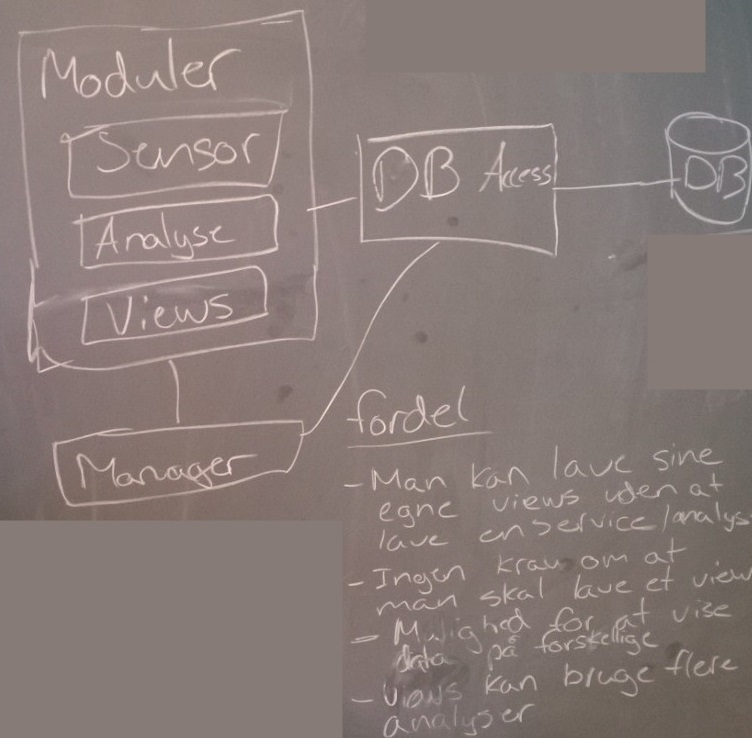
\includegraphics[width=\textwidth]{architecture_draft}
	\label{arkitektur_udkast_1}
	\caption{Første udkast til arkitektur.}
\end{figure}

\subsection*{Manager}
Denne komponent står for at holde styr på hvilke moduler der er installeret og opretter tabeller i databasen for dem.
\textit{Manageren} indeholder også et GUI så brugeren kan tilføje og fjerne moduler.
\textit{Manageren} har også logikken for hvilke \textit{analyse} moduler der kan vises i hvilke \textit{views}.
Desuden indeholder \textit{manageren} også et JSON skema for hver modul-type i \textit{moduler} komponenten.

\subsection*{Moduler}
Denne komponent består af tre lag: \textit{sensor}, \textit{analyse} og \textit{views}.
Alle moduler i hvert lag indeholder en JSON beskrivelse.

\paragraph{Sensor}
\textit{Sensor} laget indeholder alle de moduler der logger data fra sensor eller logger data fra applikationer.

\paragraph{Analyse}
\textit{Analyse} laget indeholder alle moduler der bruger et antal \textit{sensor} moduler og analyserer det data.
Dette modul foretager fx en del beregninger over tid og har et antal datatyper som output.

\paragraph{Views}
\textit{Views} laget indeholder alle moduler der gør det muligt at visualisere de analyserede data.
Den angiver hvilke og hvor mange datatyper den kan vise.

\subsection*{DB Access}
Denne komponent holder styr på hvem der skriver og læser fra databasen og på hvilken måde.

\subsection*{DB}
En sqlite database.

Vores idé til en arkitektur til systemet er som følgende:
Der er en mængde af moduler(som er uafhængige applikationer?), disse kan være sensor moduler som køre services der indsamler data om patienten, eller analyse moduler som analyserer sensor indsamlet data og tilsidst views som definerer hvordan data fra sensor og analyse moduler skal præsenteres til brugeren. Disse moduler har en interface kaldet DBAccess som giver dem adgang til databasen. Til sidst er der et manager modul som håndterer hvilke moduler skal køre og hvilke data der skal vises.

Fordelen ved denne model er at man kan lave sine egne views uden af lave en service og analyse, der er ingen krav om at man skal lave et view, man kan vise den samme data på forskellige måde og views kan bruge flere forskellige analyser.

Vi har tiltænkt det på denne måde da man skal kunne let tilføje nye moduler(ny sensor, view, analyse) til systemet, og den mest logiske måde at gøre dette på er at man kan skrive ny applikationer/moduler som så kan findes og bruges gennem managerne da det så ikke påkræver at man har adgang til det større systems kode men bare følger konventioner for hvordan man laver nye dele til det system. For eksempel en person vil gerne tilføje en temperatur sensor, men den eksisterer ikke i det originale system og han har brug for det, så han ser på guidelines til hvordan sensorer skal implementeres, skriver sit eget modul og installerer det nye modul som en applikation.

Den generelle idé bag ved arkitekturen er modularitet, altså hvor man inddeler et system i mindre dele som har sine egne ansvar som kan laves uafhængigt og genbruges i andre systemer. Altså at hvert modul indholder alt der er nødvendigt til at udføre deres opgave.

Som regel når man konstruerer et modulært system laver man mange forskellige moduler som så kompileres sammen i enden, hvor fordelen så er at man kan have flere forskellige teams som arbejder på det samme generelle system men på forskellige moduler som bare passes ind i systemet i slutningen. 

\url{http://en.wikipedia.org/wiki/Modular_design}
\url{http://en.wikipedia.org/wiki/Modular_programming}

Man bruger som regel en multi-proces arkitektur når man vil lave et robust system hvor hvis en af processerne crasher vil det ikke medfølge at hele systemet går ned, adskildning af ansvar hvor hver eneste proces har et begrænset ansvar og de ikke nødvendigvis er afhængige af andre processer i systemet, man undgår at en proces har alt for meget ansvar og skal gøre alt for meget, responsivitet af systemet, og i nogle situationer bedre sikkerhed.

Et eksempel på denne multi proces arkitektur er GIRAF(dog anerledes, hele systemet er konstrueret af en mængde af applikationer som gør noget anerledes men i den samme kontekst og samme data lager). 

Et anden eksempel på er Windows arkitekturen hvor der er flere forskellige programmer som har forskellige ansvar som sammen opgør operativ systemet. 

Et tredje er Chromium/Chrome browseren, som bruger flere processer til at sikre robusthed af systemet, da hvis det hele bare var en proces og f.eks. den del der sørger for rendering af en webside crasher vil hele systemet crashe, mens hvis hver webside har sin egen process vil et crash af en eller flere af dem ikke gøre at hele systemet crasher. De bruger også et multi-proces da det gør det mere responsivt, og giver bedre mulighed for sikkerhed da det afgrænser hvad de forskellige processer kan gøre hvis de overtages ved et angreb.

\url{http://www.chromium.org/developers/design-documents/multi-process-architecture}
\url{http://www.chromium.org/developers/design-documents/inter-process-communication}
\url{http://blog.chromium.org/2008/09/multi-process-architecture.html}

Mønstre og metoder måske relevant til et fler-applikations modulart system:

Inter-process communication som der bruges i Linux eller Windows er en måde at dele data over flere lignede eller forskellige processer i et system, dette kan f.eks. bruges til deling af information, opdeling af arbejde til forskellige dele af et system. Dette bruges tit til at opnå modularitet i et system. --- Til vores arkitektur har vi deling af information gennem en delt database som alle applikationer har adgang til, hvilket passer til IPC hvor man f.eks. kan dele en del af memory over flere processer, man kan dele filer osv. Et eksempel på dette er f.eks. D-Bus på Linux.

Chromium/Chrome bruger også IPC til at kommunikere mellem processer.

\url{http://en.wikipedia.org/wiki/Inter-process_communication}
\url{http://en.wikipedia.org/wiki/D-Bus}

Det generelle modul mønstre er mere til brug af f.eks. hvordan man skaber selvstændige dele af et program, som bliver kompileret til den samme binære fil. Dette kunne f.eks. være en singleton eller statiske klasser der har alt hvad de har brug for til at kunne udføre deres opgave. 
